%% Preambel
\documentclass[conference,compsoc,final,a4paper]{IEEEtran}
\usepackage[utf8]{inputenx}

\newcommand{\autoren}[0]{Salame, Ahmed}
\newcommand{\dokumententitel}[0]{Wieso ein gutes API Design wichtig ist}

% Hie muss normalerweise nichts angepasst werden
\usepackage[pdftex]{graphicx}
\graphicspath{{img/}}
\DeclareGraphicsExtensions{.pdf,.jpeg,.png}
\usepackage[cmex10]{amsmath}
\usepackage{algorithmic}
\usepackage{array}
\usepackage{dblfloatfix}
\usepackage{url}
\usepackage[autostyle=true,german=quotes]{csquotes}
\usepackage[backend=biber]{biblatex}
\usepackage{booktabs}
\usepackage{xcolor}
\usepackage{listings}             % Source Code listings
\usepackage[printonlyused]{acronym}

% Farben definieren
\definecolor{linkblue}{RGB}{0, 0, 100}
\definecolor{linkblack}{RGB}{0, 0, 0}
\definecolor{darkgreen}{RGB}{14, 144, 102}
\definecolor{darkblue}{RGB}{0,0,168}
\definecolor{darkred}{RGB}{128,0,0}
\definecolor{comment}{RGB}{63, 127, 95}
\definecolor{javadoccomment}{RGB}{63, 95, 191}
\definecolor{keyword}{RGB}{108, 0, 67}
\definecolor{type}{RGB}{0, 0, 0}
\definecolor{method}{RGB}{0, 0, 0}
\definecolor{variable}{RGB}{0, 0, 0}
\definecolor{literal}{RGB}{31,0, 255}
\definecolor{operator}{RGB}{0, 0, 0}

\usepackage[ngerman]{betababel}
\usepackage[
	    unicode=true,
      hypertexnames=false,
      colorlinks=true,
      colorlinks=false,
      linkcolor=darkblue,
      citecolor=darkblue,
      urlcolor=darkblue,
      pdftex
   ]{hyperref}
%	 \PrerenderUnicode{ü}

% Einstellungen für Quelltexte
\lstset{
      xleftmargin=0.1cm,
      basicstyle=\scriptsize\ttfamily,
      keywordstyle=\color{keyword},
      identifierstyle=\color{variable},
      commentstyle=\color{comment},
      stringstyle=\color{literal},
      tabsize=2,
      lineskip={2pt},
      columns=flexible,
      inputencoding=utf8,
      captionpos=b,
      breakautoindent=true,
	  breakindent=2em,
	  breaklines=true,
	  prebreak=,
	  postbreak=,
      numbers=none,
      numberstyle=\tiny,
      showspaces=false,      % Keine Leerzeichensymbole
      showtabs=false,        % Keine Tabsymbole
      showstringspaces=false,% Leerzeichen in Strings
      morecomment=[s][\color{javadoccomment}]{/**}{*/},
      literate={Ö}{{\"O}}1 {Ä}{{\"A}}1 {Ü}{{\"U}}1 {ß}{{\ss}}2 {ü}{{\"u}}1 {ä}{{\"a}}1 {ö}{{\"o}}1
}

\hypersetup{
  pdftitle={\dokumententitel},
	pdfauthor={\autoren},
	pdfdisplaydoctitle=true
}

% Wo liegt Sourcecode?
\newcommand{\srcloc}{src/}

% Literatur einbinden
\addbibresource{literatur.bib}

\begin{document}

% Titel des Dokuments
\title{\dokumententitel}

% Namen der Autoren
\author{
  \IEEEauthorblockN{\autoren}
  \IEEEauthorblockA{
    Hochschule Mannheim\\
    Fakultät für Informatik\\
    Paul-Wittsack-Str. 10,
    68163 Mannheim
    }
}

% Titel erzeugen
\maketitle
\thispagestyle{plain}
\pagestyle{plain}
 % Weitere Einstellungen aus einer anderen Datei lesen

% Eigentliches Dokument beginnt hier
% ----------------------------------------------------------------------------------------------------------

% Kurze Zusammenfassung des Dokuments
\begin{abstract}
Dieses Paper soll aufzeigen, was eine \ac{API} ist und welche Vorteile es für einen Entwickler hat. Dabei zeigt dieses Paper sowohl Kriterien eine guten API, als auch Beispiele von schlechtem API Design. Das wird mit Beispielen erläutert, z. B. anhand einer Dokumentation oder anhand dem Aufbau einer Schnittstelle. Des Weiteren werden verschiedene Ansätze aufgezeigt, wie eine nutzerfreundlichere API entworfen werden kann. Es werden Tools vorgestellt, welches die Wartung einer API erleichtern und potenzielle Fehler minimieren. Zudem wird auch auf Ansätze eingegangen, die dabei helfen, die bestehende API zu verbessern.
\end{abstract}

\tableofcontents

\section{Einleitung}

Application Programming Interfaces (API) sind kaum wegzudenken. So gut wie alle Programmbibliotheken, Frameworks und \ac{SDK} nutzen eine API. Auf der Webseite programmableweb\footnote{https://www.programmableweb.com/} werden allein über 18.000 unterschiedliche APIs aufgelistet. Abbildung \ref{apiOrte} zeigt die Vielseitigkeit einer API auf

Für die Entwicklung neuer APIs gibt es einen immer größer werdenden Markt für Firmen, die aktiv ihre Dienste zur Verfügung stellen, um Unternehmen bei der Entwicklung einer API zu unterstützen, wie z. B. Apigee \footnote{https://apigee.com/api-management/}.

Zudem besitzen Firmen unterschiedliche Strategien, wie sie mit ihrer API vorgehen. \cite[siehe Seite 11]{spichale2017}. So hat der Blogging-Dienst Twitter seine Popularität unter anderem mithilfe der hauseigenen API erreicht. Es bot die notwendige Infrastruktur, sodass Twitter auf unzähligen Endgeräten genutzt werden konnte. Facebook setzt mit seiner API auf Ausfallsicherheit und Skalierbarkeit. Die Firma Best Buy entwickelte eine API, um ihren Online-Dienst weiter auszubauen. 


\section{Application Programming Interface}

In diesem Kapitel wird vorgestellt, was eine \ac{API} ist. Es wird auf die Definition einer API eingegangen. Zudem werden die Vorteile einer API genauer erläutert. 

\begin{figure*}[h]\label{apiOrte}
\centering
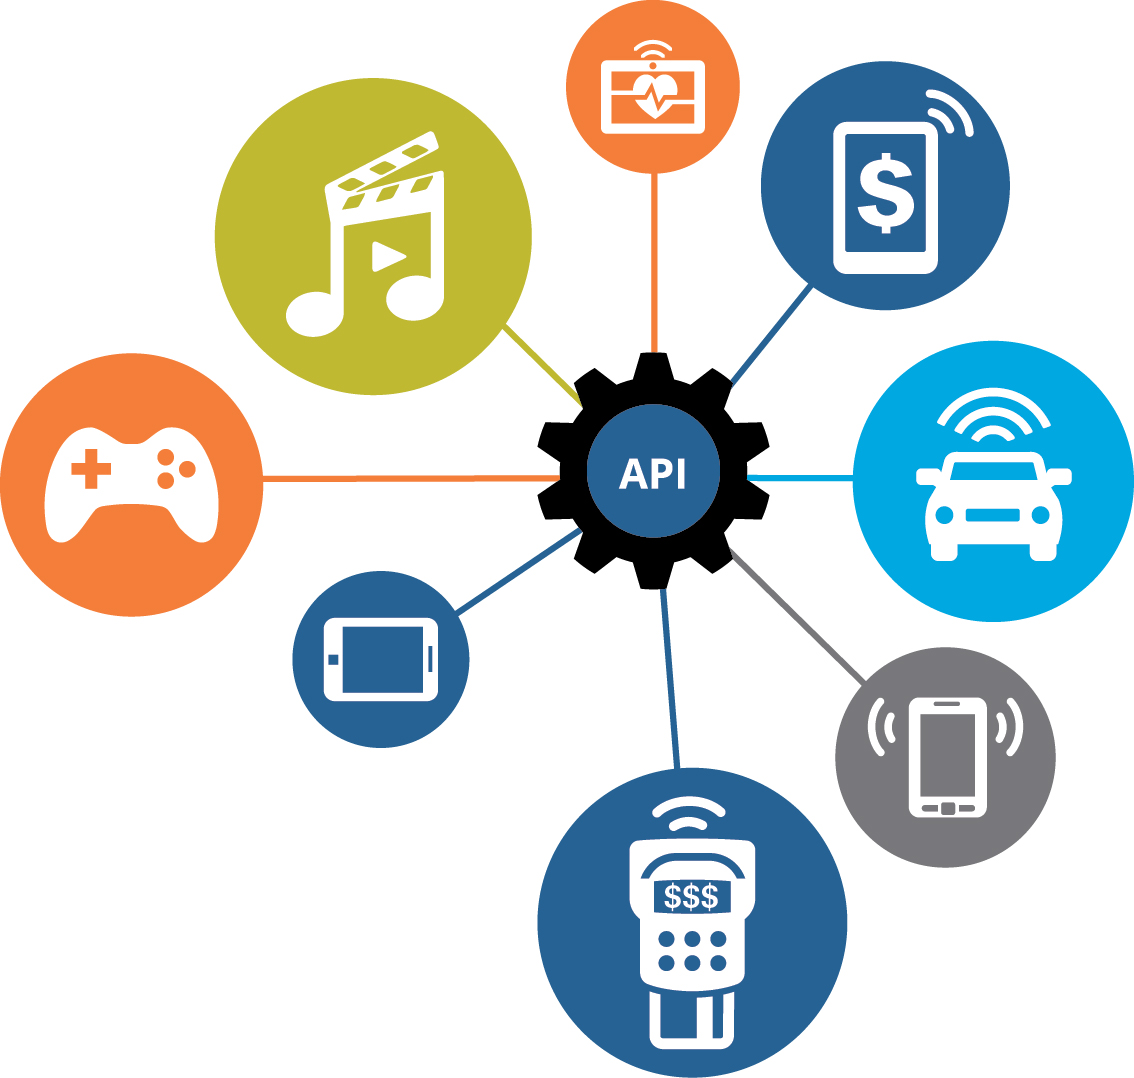
\includegraphics[,width=\textwidth,height=8cm]{api_beispiel.jpg}
\caption{Einsatzorte einer API} \protect\footnotemark
\label{apiOrte}
\end{figure*}
\footnotetext{http://www.arxan.com/wp-content/uploads/2016/07/api-protection-1.jpg}

\subsection{Die Definition einer \ac{API}}

Eine \ac{API} besitzt keine einheitliche Definition. Die unterschiedlichen Erklärungsansätze weichen an bestimmten Punkten voneinander ab. So beschreibt Reddy \cite{reddy2011}, dass eine API Schnittstellen hat, die eine Abstraktion eines Problems darstellen und wie Entwickler diese nutzen, um das bestehende Problem zu lösen.
Blochs Definition ist dabei etwas Allgemeiner \cite{bloch2014}. Laut Bloch handelt es sich um eine \ac{API}, wenn folgende Kriterien erfüllt sind:
\begin{enumerate}
\item Eine API bietet eine Menge an Operationen an, welche durch ihre Eingaben und Ausgaben definiert sind.\\
\item Es ist möglich die Schnittstellen neu zu implementieren, ohne dass der Nutzer seinen Code anpassen muss.
\end{enumerate}

Allgemein kann eine \ac{API} als etwas beschrieben werden, das dem Nutzer zur Verfügung gestellt wird, sodass dieser darüber mit einem Softwaresystem kommunizieren kann.
Im folgenden Paper wird diese Definition zugrunde gelegt.\\
Folgende beispielhafte Java Methode soll verdeutlichen, wie eine Schnittstelle konkret aussehen kann:

\begin{lstlisting}[language=Java,caption=Beispiel einer Schnittstelle in Java]

public String linkStrings(String head , String tail);

\end{lstlisting}

Der Name der Schnittstelle, die auch eine Methode ist, lautet linkStrings, ihre Eingaben sind zwei Strings, mit den Bezeichnern \textit{head} und \textit{tail}. Bei der Ausgabe der Methode handelt es sich um den Rückgabewert, welcher in diesem Fall als Typ auch vom Typ String ist. Die eigentliche Implementierung ist dabei für den Nutzer, der diese Schnittstelle nutzt, nicht relevant. Der Nutzer benötigt zur Nutzung der Schnittstelle ausschließlich die Schnittstelle selbst. Dessen Implementierung kann sich an einer anderen Stelle befinden.

\subsection{Die Arten einer API}

Es gibt unterschiedliche Arten einer API \cite{myers2016}. Es ist möglich eine API grob in drei Kategorien einzuteilen. Interne APIs sind nicht für die Öffentlichkeit gedacht. Sie werden intern verwendet und sind daher nicht auf die Akzeptanz der Community angewiesen. Dies sorgt dafür, dass interne APIs nicht denselben strengen Regeln unterliegen sind, die für öffentliche API gelten. Das bedeutet, dass diese API noch nicht von unzähligen Nutzern genutzt wird, sondern nur die Entwickler, die an dieser API selbst mitwirken. Daher ist es möglich Änderungen an der Schnittstelle vorzunehmen, ohne irgendwelche Nutzer möglicherweise zum Ändern ihres Codes zu zwingen. Sie helfen dabei, interne Strukturen umzusetzen, die das Arbeiten in verschiedenen Teams ermöglichen. 

Öffentliche APIs sind der Öffentlichkeit zugänglich. Sobald eine API öffentlich verfügbar ist, ist es kaum möglich diese so abzuändern, dass kein Nutzer dieser API seinen Code anpassen muss. Zu einer guten öffentlichen API gehört auch eine dazu passende Dokumentation. Beispiele hierfür wäre das \ac{JDK} oder die \ac{STL} von C.

Neben der öffentlichen und internen API gibt es noch die remote APIs. Hier werden die Schnittstellen über das Netzwerk zugänglich gemacht. Für den Nutzer soll dabei der Eindruck entstehen, als würde sich die API lokal befinden und nicht in einem anderen System. Der Aufruf über das Netzwerk soll dabei verborgen bleiben. Beispiel hierfür wäre die remote API von Java.


\subsection{Die Vorteile einer API}

Es gibt viele gute Gründe, die für das Erstellen einer \ac{API} sprechen. Nach Reddy \cite{reddy2011} sprechen insbesondere folgende Gründe für das entwickeln einer API:

\begin{description}
\item [Robustheit] \hfill \\

Eine \ac{API} sorgt für robusteren Code. Da die Entwickler nur über eine Schnittstelle mit dem System kommunizieren, entsteht eine Datenkapselung. Es sorgt dafür, dass die eigentliche Implementation ausgetauscht werden kann, ohne dass es beim Nutzer angepasst werden muss. So lässt sich ganz leicht die bestehende Implementierung austauschen, ohne dass der Nutzer gezwungen ist seinen Quellcode anzupassen. Es lässt sich somit z. B. ein Algorithmus durch einen besseren Algorithmus austauschen.\\

\item [Parallele Entwicklung]\hfill \\

Wenn ein Entwickler, bei der Implementierung eines Programms den Quellcode von einem seiner Kollegen benötigt, dieser allerdings den Quellcode noch nicht fertiggestellt hat, würde eine Wartezeit entstehen. Es müsste solange gewartet werden, bis der benötigte Quellcode fertiggestellt ist. Es führt zu einem immensen Zeitgewinn, wenn sich stattdessen beide einigen würden, wie die Schnittstellen definiert werden soll. So könnte vor der Implementierung der Schnittstellen ein Mockup erstellt werden, sodass sich der Quellcode  compilieren lässt. Die eigentliche Implementierung der Schnittstellen kann so später stattfinden, sodass der Nutzer dieser Schnittstelle nur wenige, bis keine Änderung vornehmen muss.

So lässt es sich realisieren, dass mehrere Teams parallel entwickeln können, ohne jedes Detail von den Aufgaben der anderen Teams zu kennen.\\
	
\item [Wiederverwendbarkeit]\hfill \\
	
Einer der größten Vorteile einer API ist die Wiederverwendbarkeit von bereits existierendem Quellcode. Das Entwickeln von eigenen Schnittstellen und dessen Implementierungen kostet sehr viel Zeit.

Durch das Wiederverwenden einer \ac{API}, kann sehr viel Geld gespart werden. Dabei stehen sowohl kostenpflichtige, als auch kostenlose zur Auswahl. Es existieren viele unterschiedliche \ac{API}s für die unterschiedlichsten Probleme.

Es gibt z. B. viele APIs, die sich mit dem Laden von Bildern beschäftigen  \footnote{http://cimg.eu/}. Viele solcher Bibliotheken haben bereits einen gewissen Reifeprozess durchlaufen. Sie wurden ausgiebig getestet und haben auch ein breites Spektrum an Dokumentationen. Als Beispiel ist hier die Spielebibliothek LibGDX zu nennen. Sie hat eine große Community, an die sich Entwickler wenden können, falls sie Fragen haben \footnote{http://www.badlogicgames.com/forum/}.
\end{description}


\section{Beispiele von schlechtem API design}

Es gibt viele Programmbibliotheken, die sehr viele Schnittstellen anbieten, auf welche die Entwickler Zugriff haben. Bei einer Erweiterung der Bibliothek kommen zudem immer mehr Schnittstellen hinzu. Wo sich noch in \ac{JDK} aus Java 8 4240 Klassen befinden \footnote{https://docs.oracle.com/javase/8/docs/api/}, hat dessen Nachfolger Java 9 bereits 6005 Klassen \footnote{https://docs.oracle.com/javase/9/docs/api/}. Bei einer solch wachsenden Anzahl an Klassen ist es wichtig, sich ein Konzept auszudenken, damit der Nutzer bei einer Bibliothek keine Schwierigkeiten bekommt. Wenn einzelne Punkte nicht eingehalten werden, kann der Nutzer schnell den Überblick verlieren. Der Erfolg einer Bibliothek kann unter anderem dadurch gemessen werden, wie häufig die Bibliothek von verschiedenen Entwicklern genutzt wird. In diesem Kapitel werden Punkte genannt, die den Erfolg einer Bibliothek bestimmen können.


\subsection{Mangelnde Dokumentation}\label{MD}

Die Dokumentation einer Bibliothek beschreibt ihre Funktionalität, auf die der Nutzer zugreifen kann. So werden die Schnittstellen einer Bibliothek in der Dokumentation definiert, sowie mit einer zusätzlichen Beschreibung versehen. Zusätzlich kann eine Dokumentation noch weitere Punkte beinhalten, wie Namenskonventionen oder Beispiele, wie die API genutzt werden kann. Ein bekanntes Beispiel hierfür ist die Java Dokumentation von Oracle. Hier werden alle Klassen, auf die der Nutzer Zugriff hat, angezeigt. Neben den Beschreibungen der Klassen, gibt es in der Java API Dokumentation auch die Beschreibungen für die Methoden der Klassen.

Für das Erstellen von Dokumentationen gibt es viele Möglichkeiten. Die Programmiersprache Java bietet für die Dokumentation des Quellcodes das Javadoc an \cite{oracle2017}. Bei Javadoc handelt es sich um ein Tool für das Generieren von API Dokumentation. Dabei braucht ein Entwickler z. B. über einer Methode nur ein Javadoc Kommentar zu schreiben, sodass das Javadoc Tool es in \ac{HTML} Code umwandeln kann. Beim Javadoc Kommentar lassen sich auch die Abhängigkeiten als Referenzen zu anderen Klassen und Methoden herstellen. Das erleichtert dem Nutzer zusätzlich die Suche nach der benötigten Klasse, da der Nutzer per Mausklick die benötigte Seite im \ac{HTML} aufrufen kann. Die Java API Dokumentation selber wurde mithilfe von Javadoc erstellt. Listing 2 zeigt eine Methode mitsamt deren Javadoc aus der java.lang.String Klasse gezeigt:

\begin{lstlisting}[language=Java,caption=Beispiel eines Javadoc Kommentars]

  /**
  * Returns the {@code char} value at the
  * specified index. An index ranges from {@code 0} to
  * {@code length() - 1}. The first {@code char} 
  * value of the sequence
  * is at index {@code 0}, the next at index {@code 1},
  * and so on, as for array indexing.
  *
  * <p>If the {@code char} value specified by the 
  * index is a
  * <a href="Character.html#unicode">surrogate</a>, 
  * the surrogate
  * value is returned.
  *
  * @param      index   the index of the {@code char} 
  * 					value.
  *
  * @return     the {@code char} value at the specified 
  *				index of this string.
  *             The first {@code char} value is at 
  *				index {@code 0}.
  *
  * @exception  IndexOutOfBoundsException  if 
  *				the {@code index}
  *             argument is negative or not less than 
  *				the length of this string.
  */
 public char charAt(int index) {
     if ((index < 0) || (index >= value.length)) {
         throw 
         	new StringIndexOutOfBoundsException(index);
     }
     return value[index];
 }

\end{lstlisting}

Auch andere Bibliotheken, die in Java geschrieben worden sind, haben so ihre Dokumentation erstellt. Zu nennen wäre hier z. B. die Bibliothek \ac{LWJGL} \footnote{https://javadoc.lwjgl.org/} oder die Spielebibliothek LibGDX \footnote{https://libgdx.badlogicgames.com/nightlies/docs/api/}. Das Javadoc nimmt beim Erstellen des Quellcodes viel Arbeit für eine externe Dokumentation ab. 

Ein ähnliches Tool für das Erstellen einer Dokumentation ist Doxygen \cite{dimitri2017}. Doxygen steht dabei nicht nur für Java zur Verfügung, sondern auch für andere Programmiersprachen wie C, C++ oder Python. Wie in Javadoc wird auch hier die Dokumentation über Kommentare im Quelltext gesteuert, allerdings hat der Entwickler in Doxygen die Möglichkeit die Dokumentation in verschiedenen Arten anzugeben \footnote{https://www.stack.nl/~dimitri/doxygen/manual/docblocks.html}. Es ist zudem möglich, mit Doxygen einen zusammenfassenden Überblick über den Aufbau des Projektes zu erzeugen. Doxygen als Erweiterung wird von vielen Entwicklungsumgebungen [Abschnitt \ref{IDE}] unterstützt. Des Weiteren unterstützt Doxygen eine einfache Syntaxhervorhebung für die Übersicht. 

Der Vorteil einer Dokumentation, welche im Quelltext beschrieben wird, ist die geringere Fehleranfälligkeit im Vergleich zu extern erstellten Dokumentationen. Eine externe Dokumentation müsste immer separat angepasst werden, falls Änderungen getätigt werden. Zudem ist die Pflege im Quelltext einfacher. 


\subsection{Keine eindeutigen Bezeichnungen von Schnittstellen}

Falls eine Dokumentation die API nicht gut genug dokumentiert, sodass z. B. eine Schnittstelle nicht genau genug beschrieben wurde, wie sie konkret funktioniert und von was sie abhängig ist, kann es dazu führen, dass ein Entwickler eine Schnittstelle der API falsch nutzt.  

%Negatives Beispiele
Die Java Klasse java.util.Calendar \footnote{https://docs.oracle.com/javase/7/docs/api/java/util/Calendar.html} besitzt folgende Methode:

\begin{lstlisting}[language=Java,caption=Signatur der Methode set]

public final void set(int year, int month, int date)

\end{lstlisting}

Anhand der Parameter wäre es naheliegend, dass beim Aufruf mit dem folgenden Werten die Methode das Datum auf den 22 August 2017 setzt:

\begin{lstlisting}[language=Java,caption=Setzten eines Datums]

Calendar cal = Calendar.getInstance();

cal.set(2017, 8, 22);

\end{lstlisting}

Allerdings ist anhand der Beschreibung der Methode erkenntlich dass bei der Eingabe vom Monat, der Januar nicht mit der Eins, sondern mit der Null beginnt. Also wäre das Datum, welches im obigen Beispiel gesetzt wurde, der 22 September 2017. Vorgesehen ist, dass Setzen des Datums folgendermaßen zu machen:

\begin{lstlisting}[language=Java,caption=Setzten eines Datums mit Konstante]

Calendar cal = Calendar.getInstance();

cal.set(2017, Calendar.AUGUST, 22);

\end{lstlisting}

Es wird keine Zahl der Methode als Monat übergeben, sondern eine Konstante. Auch wenn die Methode set dokumentiert ist, so legt die Benennung ihrer Parameter nahe, dass der Nutzer beim Nutzen dieser Methode einfach Zahlen übergeben kann, sodass der Nutzer die Dokumentation nicht zu lesen braucht. Tatsächlich soll laut Bloch \cite{bloch2006} eine Methode so definiert sein, dass es einfach ist diese Methode zu nutzen, aber es schwierig ist, diese Methode falsch zu nutzen. Idealerweise wird im Vorfeld verhindert, dass die Methode falsch genutzt werden kann. Zudem soll die Methode einer API nicht zwangsweise dokumentiert sein, wenn der Bezeichner der Methode und ihre Parameter die Funktionsweise nahelegen. 

Ein anderes Beispiel für eine Methode, die missverstanden werden kann \cite[ab Minute 7]{bloch2009}, ist folgende Methode:

\begin{lstlisting}[language=Java,caption=getBoolean Methode aus java.lang.Boolean]

public static boolean Boolean.getBoolean(String name);

\end{lstlisting}

Sie stammt aus der Klasse java.lang.Boolean \footnote{https://docs.oracle.com/javase/9/docs/api/java/lang/Boolean.html}. In Java gibt es sogenannte Wrapperklassen. Sie stellen Repräsentanten der primitiven Datentypen als Klassen dar, wie int, double oder auch boolean. Daher gibt es jeweils für jeden primitiven Datentyp eine Wrapperklasse, für den Datentyp int wäre es z.B. java.lang.Integer. Jede Klasse besitzt mindestens eine Methode, dessen Bezeichner mit get anfängt, wie z. B. getInteger oder wie im Beispiel getBoolean. Es liegt nahe, dass viele Entwickler zunächst annehmen würden, dass beim Aufruf der Methode getValue der Wert true geliefert wird.

\begin{lstlisting}[language=Java,caption=Beispiel mit getValue]

public static boolean getValue(){
	
	boolean bol = Boolean.getBoolean("true");

	if(bol == true){

		return true;

	}else{

		return false;
	
	}
	
}

\end{lstlisting}

Allerdings wird hier false geliefert. In der Dokumentation dieser Methode ist zu entnehmen, dass die Methode getBoolean nur dann true liefert, falls es ein System Property gibt, welches den Namen trägt, der übergeben wird, und den Wert true oder TRUE zugewiesen bekommen hat:

\begin{lstlisting}[language=Java,caption=Beispiel mit getValue mit vorher gesetztem Propertie]

public static void main(String[] args) {

	Properties properties = new Properties();

	properties.setProperty("TRUE", "true");

	System.setProperties(properties);

	System.out.println(getValue("TRUE")); 

}

public static boolean getValue(String str) {

	boolean bol = Boolean.getBoolean(str);

	if (bol == true) {

		return true;

	} else {

		return false;

	}

}

\end{lstlisting}


Diese Vorgehensweise ist irreführend, da von dem Bezeichner der Methode nicht hervorgeht, dass vorher die System Property gesetzt werden muss.


\subsection{Factory Pattern mit Bedacht einsetzen}

Das Factory Pattern ist ein Entwurfsmuster, welches von der Gang of Four im Buch Design Pattern  \cite{gamme1995} beschrieben wird. Das Pattern wird dazu genutzt, dass der Nutzer, um eine Klasse zu instanziieren, es nicht über den Konstruktor tätigt, sondern über eine Methode. Der Entwickler soll so nicht mit dem Konstruktor in Berührung kommen. Es hat insbesondere den Vorteil, dass es so möglich ist, den Typ eines Objektes zur Laufzeit zu bestimmen.
Folgender Codeausschnitt soll eine beispielhafte Implementierung in Java zeigen:

\begin{lstlisting}[language=Java,caption=Beispiel eines Factory Patterns in Java]

public class Factory
{
    public static Base factoryMethod(int typeNumber)
    {
        switch (typeNumber)
        {
            case 1: return new ConcreteProduct1();
            case 2: return new ConcreteProduct2();
            default: throw new ArgumentException("Invalid type.", "type");
        }
    }
}
 
public abstract class Base { }
 
public class ConcreteBase1 extends Base { }
 
public class ConcreteBase2 extends Base { } 

\end{lstlisting}

In dem obigen Code.Beispiel werden über die Klasse Factory, die Objekte für die Klasse ConcreteBase1 und ConcreteBase2 erzeugt. So kann der Entwickler Objekte der Klasse nicht nur über den Konstruktor der Klasse erzeugen, sondern auch vorgefertigte Instanzen über die statische Methode factoryMethod in der Klasse Factory. So muss sich der Entwickler keine Gedanken machen, welche Parameter der Konstruktor benötigt, falls dieser welche hat.

Auch wenn das Factory Pattern dem Entwickler es scheinbar einfacher macht an Objekte von einem bestimmten Typ zu kommen, sollte das Factory Pattern nur bedacht eingesetzt werden. 
In einer empirischen Studie von Ellis \cite{ellis2007} wurde der Unterschied zwischen einer API die Konstruktoren nutzt und einer API die das Factory Pattern nutzt untersucht. Diese Studie kam zum Schluss, dass das Factory Pattern wohl weniger geeignet ist im Gegensatz zu anderen Patterns, wie das Class Cluster Pattern. 


\section{Ansätze zur Verbesserung allgemeiner \ac{API}s}

Eine API bietet viele Möglichkeiten für eine stetige Verbesserung. Eine API, die öffentlich genutzt wird, hat meist viele Schritte zur Verbesserung durchgemacht. Die Schritte zur Verbesserung einer API kann sich dabei auch über Jahre strecken. Jedoch muss das Resultat nicht zwingend in jedem Fall positiv sein \cite[siehe Seite 25]{spichale2017}.

Im Folgenden werden einige Vorgehensweisen beschrieben, die aufzeigen sollen, wie dafür gesorgt werden kann, dass eine API auch einer konsequente Verbesserung widerfährt.


\subsection{Nutzerfreundlicheres Design}

Viele Entwickler, die mit wenig benutzerfreundlichen APIs arbeiten, können große Probleme haben diese API zu erlernen. Nach Robillards Untersuchung haben die Entwickler folgendes angegeben \cite{robillard2009}:
\begin{itemize}
\item 78 Prozent gaben an, eine API durch ihre Dokumentation zu lernen.
\\
\item 55 Prozent gaben an, eine API durch Code Beispiele zu lernen
\\
\item 34 Prozent gaben an, eine API zu lernen, indem sie damit herumexperimentieren, um 			so ein die Funktionsweise zu verstehen.
\\
\item 30 Prozent gaben an, dass sie sich von ihren Kollegen einweisen lassen.
\\
\item 29 Prozent gaben an, dass sie sich Artikel zu den API durchlesen
\end{itemize}

Anhand der Ergebnisse sieht man ziemlich gut, wie wichtig eine Dokumentation für die Nutzer einer API ist. Mehr als drei Viertel gaben an, dass sie sich erst in die Dokumentation einlesen, bevor sie mit der API programmieren. Daher kann es essenziell sein, mit der API auch eine gute Dokumentation zu haben. Mehr als ein Drittel geben an, eine API zu lernen indem sie mit dessen Schnittstellen herumexperimentieren. Daraus ist zu entnehmen, dass ein verständliches Design der Schnittstellen für viele Entwickler das Mittel ist, um diese API zu lernen. Zudem gaben die Testpersonen an, dass es für sie auch wichtig sei, dass die Dokumentation einige gute Beispiele beinhalten soll. So z. B. komplexere Szenarien, die mit Code Beispielen untermauert werden. Auch eine strukturierte Ordnung sei wichtig. 

\subsection{APIs Testen}

Um die Qualität einer API zu verbessern, ist es sinnvoll die API vorher zu testen. Neben den Unit-Tests \footnote{https://martinfowler.com/bliki/UnitTest.html}, gibt es auch Testmöglichkeiten, bei denen es von einem Entwickler getestet wird. Der Zweck von diesen Tests ist es, die Benutzerfreundlichkeit der APIs zu erhöhen. 

Es bieten sich für menschliche Tests einige Möglichkeiten an. Eine davon ist das Peer-Reivew \cite{farooq2010}. Das Ziel einer API Peer-Review ist es, Rückmeldung zu erhalten, wie stark die Benutzerfreundlichkeit der API ist. Hier werden eine oder mehrere Personen damit beauftragt, die Schnittstellen zu begutachten.

\section{Ausgewählte \ac{API} Entwurfsmuster}

Bloch beschreibt die Eigenschaft einer guten API folgendermaßen:
\\\\
Good APIs create long-term customers; bad ones create long-term support nightmares\cite{bloch2006}.
\\\\
Eine API, die nutzerfreundlich ist, erspart einem Entwickler, der diese API nutzt, sehr viel Stress und vor allem Zeit. Auch ist das Design entscheidend für den Erfolg einer API. Viele Entwurfsmuster haben sich dabei durchgesetzt, mit dessen Hilfe eine API dahingehend verbessert werden kann, dass es dem Entwickler, welcher mit der API arbeiten muss, das Leben erleichtert.

Im Folgenden werden einige Entwurfsbeispiele für eine API aufgezählt.


\subsection{Sinnvolle Klassennamen wählen}

In objektorientierte Programmiersprachen, wie Java oder C++, sind die Namen der Klassen ebenso relevant, wie die Methodennamen. Ein wesentlicher Grund dafür ist, dass hierbei die Objekte Schnittstellen nach außen anbieten, auf die dann der Nutzer dieser API Zugriff hat. Zudem sind viele Objekte, sei es durch Vererbung oder durch eine Parameterübergabe an eine Methode, miteinander verbunden. 
Der Name einer Klasse sollte ein Substantiv sein \cite{martin2009}. Er sollte zudem mit einem großen Buchstaben anfangen. Einige Beispiele für gute Klassennamen wären:

\begin{lstlisting}[language=Java,caption= Klassennamen]

public class Human{...}

public class Customer{...}

public class Applikation{...}

public class Number{...}

\end{lstlisting}

Das Verwenden eines Substantivs in einem Klassennamen vereinfacht für den Nutzer die Suche nach einer Schnittstelle, die sich in einer naheliegenden Klasse befindet.
Ein guter Klassenname bezieht sich immer auf den Typen, den diese Klasse darstellen soll. Daher sollte der Klassenname nicht von der technischen Implementierung abhängig sein. 

\subsection{Methodennamen und ihre Parameter}\label{MNP}

Der Name einer Methode, und damit auch die der Schnittstelle, sollte idealerweise ihren Zweck beschreiben. Einen passenden Namen für eine Methode zu wählen, kann viel Zeit kosten, allerdings erleichtert es dem Nutzer, die ansonsten zeitaufwendige Suche nach einer passenden Methode \cite[siehe Seite 45f]{martin2009}.

Wenn sich ein Entwickler in eine neue Bibliothek einarbeiten soll, dann gibt es hierfür verschiedene Ansätze. Ein erster Ansatz wäre, dass er die Dokumentation der Schnittstellen der Bibliothek durchgeht [Abschnitt \ref{MD}]. Nach Martin ist eine Dokumentation allerdings kein Ersatz für die Bezeichner einer Schnittstelle. Martin zufolge ist es sogar so, dass eine Schnittstellen-Dokumentation ein Zeugnis dafür, dass der Entwickler dieser Schnittstelle nicht imstande war, bessere und selbsterklärendere Methodennamen zu verwenden. Das Resultat dieser Aussage ist, dass eine Schnittstelle sich demnach selbst beschreiben soll, sodass eine Dokumentation nicht erst notwendig ist. 

Nach Martin \cite[siehe Seite 51f]{martin2009} ist daher beim Design einer API, für die Schnittstellen Namen zu wählen, nach denen der Nutzer einfacher suchen kann. Zudem sind auch Namen besser geeignet, die je nach Umfang der Schnittstelle eine entsprechende Länge haben. 
Dadurch kann der Entwickler intuitiv nach einer Methode suchen, indem er nach dem Bezeichner der Methode sucht. Einige Entwicklungsumgebungen, wie z. B. Eclipse oder Microsoft Visual Studios, beinhalten Funktionen, die unter anderem das Suchen von Methoden beinhalten \footnote{http://help.eclipse.org/kepler/index.jsp Begriff: Java Search Tab} \footnote{https://blogs.msdn.microsoft.com/visualstudio/2010/01/13/searching-and-navigating-code-in-visual-studio-2010/}. Dabei ist es nicht notwendig nach dem vollen Namen der Methode zu suchen, es genügen auch einzelne Wortteile. Die Entwicklungsumgebung übernimmt dann die Suche und listet alle verfügbaren Methoden auf, die dieses Wortteil beinhalten.

Abbildung \ref{suchoption} zeigt einen Bildausschnitt aus der Suchoption von Eclipse, Abbildung \ref{suchergebniss} zeigt dessen Suchergebnis. Daher ist es einfacher für den Nutzer sich in einer API zurechtzufinden, wenn dessen Schnittstellen einer gewissen Konvention folgen \cite{haase2015}. Sobald sich ein Nutzer in eine API eingearbeitet hat, entwickelt er eine gewisse Routine. \cite[siehe Seite 14f]{martin2009}.

\begin{figure*}[h]
\centering
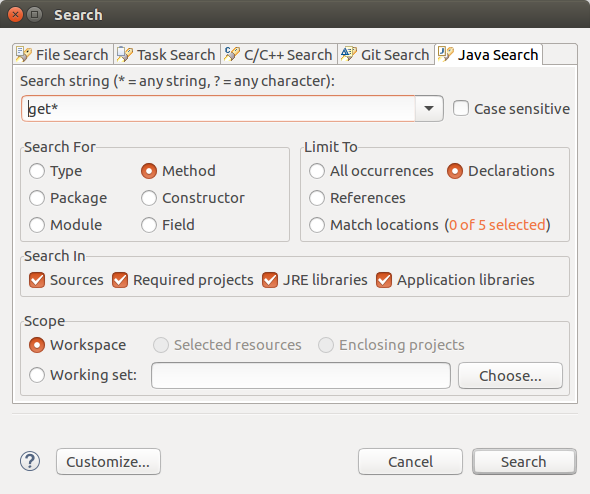
\includegraphics[,width=\textwidth,height=10cm]{eclipse_suche.png}
\caption{Suchoption aus Eclipse}
\label{suchoption}
\end{figure*}

\begin{figure*}[h]\label{suchergebniss}
\centering
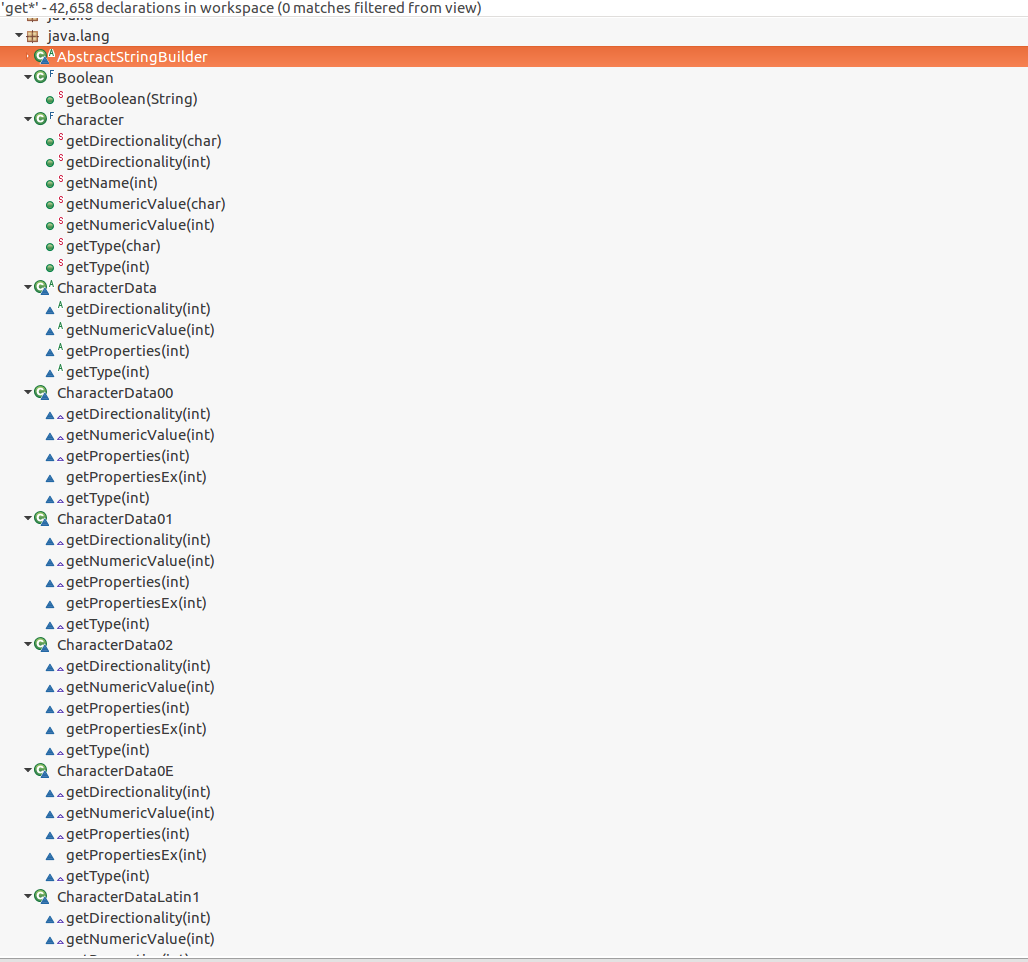
\includegraphics[,width=\textwidth,height=8cm]{eclispe_suche_ergebniss.png}
\caption{Suchergebnis aus Eclipse}
\label{suchergebniss}
\end{figure*}

\subsection{Refactoring}\label{refactorL}

Das Refactoring beschreibt laut Fowler einen Prozess, bei dem bestehender Quellcode so verändert wird, dass die Änderung keinen Einfluss auf die eigentliche Funktion hat. \cite{fowler1999}. Mit dem Refactoring wird versucht bestehenden Quellcode so zu verbessern, dass die Chancen für mögliche Programmfehler minimiert werden. Zudem wird meist zusätzlich auch der Quellcode verbessert, sodass es besser lesbar und somit wartbar ist. Nach Fowler ist das Refactoring keine zusätzliche Arbeit, sondern ein fester Bestandteil bei der Software-Entwicklung.

Auch wenn ein gutes Design der API vorliegen sollte, kann es bei zusätzlichen Erweiterungen dazu kommen, dass die Schnittstellen nicht mehr nach dem ursprünglichen Design entworfen worden sind. Dies könnte dazu führen, dass eine Namenskonventionen nicht eingehalten worden sind \ref{MNP}. Es kann auch vorkommen, dass die Parameternamen einer Methode nicht aussagekräftig genug sind und dies für den Nutzer zur Verwirrung führen könnte. Falls die API noch nicht veröffentlicht wurde, ist es zudem auch möglich die Schnittstellen selber in den Refactoring Prozess einzubinden und sie zu verändern.

Das Refactoring kann dazu genutzt werden, solche Missstände auszubessern und den Quellcode leserlicher zu machen. Zudem kann es auch den Stress für den Nutzer dieser API minimieren. 
 
Als Beispiel soll folgende, sehr simple gehaltene, Schnittstelle dienen:
 
\begin{lstlisting}[language=Java,caption=Beispiel einer schwer zu lesende Methode]

public int[] fusion(int[] a, int[] b);

\end{lstlisting}

Die Methode soll zwei Arrays miteinander kombinieren. Das Array mit dem Namen b soll an a angehängt werden. Das kombinierte Array wird dann zurückgegeben. Der Name der Methode lautet fusion und bekommt zwei Arrays mit den nichtssagenden Namen a und b. Es lässt sich nicht eindeutig sagen, was diese Methode genau bewirkt. 

Mithilfe von Refactoring lässt sich diese Methode so abändern, dass auch alle weiteren vorkommenden dieser Methode angepasst werden. Bei dem Namen fusion kann es zu einem Missverständnis beim Entwickler kommen. So ist es möglich, dass der Entwickler annimmt, dass der Inhalt beider Arrays jeweils miteinander addiert wird. 

Der Name der Methode kann mithilfe von Refactoring abgeändert werden, unabhängig von der Funktionsweise der Methode. Es wäre also möglich die Methode folgendermaßen zu benennen:

\begin{lstlisting}[language=Java,caption=Beispiel einer Methode mit unverständlichen Parametern]

public int[] combine(int[] a, int[] b);

\end{lstlisting}

Mit dem Namen wäre diese Methode nun deutlich lesbarer für den Nutzer dieser API. Allerdings könnte es aufgrund der Parameterbenennung zu Unklarheiten kommen. Es ist nicht eindeutig ersichtlich, ob b an a angehängt wird oder andersherum. Es wäre mithilfe von Refactoring möglich beide Parameter so umzubenennen, sodass ihre Namen ihre Rolle klar hervorheben. Auch hier wäre es nicht notwendig, in der Implementierung die Namen anzupassen:

\begin{lstlisting}[language=Java,caption=Beispiel einer leserliche Methode]

public int[] combine(int[] head, int[] tail);

\end{lstlisting}

Nun ist ersichtlich, wie genau beide Arrays miteinander kombiniert werden. Das erleichtert dem Nutzer 

Das Refactoring ist eine immense Zeitersparnis, bei dem Verbessern der bestehenden Schnittstelle. Dies ist allerdings nur 

\section{Tools zur Unterstützung der Entwicklung einer API}

Das Programmieren und Testen können die Entwicklung einer API sehr langwierig machen. Viele Bibliotheken haben mehrere tausende Schnittstellen, was zu sehr unübersichtlichen Quellcode führen kann. Es gibt allerdings viele Tools, die einem das Arbeiten erleichtern. Im Folgenden werden einige Tools vorgestellt und deren Vorteile dargestellt. 


\subsection{Entwicklungsumgebung}\label{IDE}

Es gibt sehr viele Entwicklungsumgebungen, mit deren Hilfe das Programmieren erleichtert wird. Einer der bekanntesten Vertreter wäre Microsoft Visual Studio \footnote{https//www.visualstudio.com/}. Microsoft bietet mehrere Versionen seiner Entwicklungsumgebung Visual Studio, zum einen als kostenpflichtige Premium Edition und zum anderen als kostenlose Community Edition. Sie bietet Unterstützung für viele verschiedene Programmiersprachen, wie C, C++, C\#, Javascript oder Python.
 
Neben der Entwicklungsumgebung von Microsoft gibt es auch noch IntelliJ von JetBrains  \footnote{https://www.jetbrains.com/idea/}. Ähnlich wie Microsofts Visual Studio bietet IntelliJ Sprachunterstützung für viele verschiedene Programmiersprachen an. Auch gibt es hier sowohl eine kostenpflichtige als auch eine Community Version. Im Gegensatz zu Microsoft Visual Studio ist IntelliJ auch außerhalb von Microsoft Windows verfügbar. 

Die beliebteste Entwicklungsumgebung laut \ac{PYPL} ist das in Java geschriebene Programm Eclipse von Eclipse Software \footnote{http://www.eclipse.org/} \footnote{http://www.eclipse.org/}. Auch Eclipse erlaubt mithilfe von Erweiterungen eine Sprachunterstützung von unterschiedlichen Sprachen, ursprünglich war sie dabei allerdings nur für die Programmiersprache Java gedacht. All die genannten Entwicklungsumgebungen unterstützen das Refactoring [Abschnitt \ref{refactorL}]. 

Entwicklungsumgebungen sind eine große Hilfe beim Entwickeln und Verbessern einer API. Da die Entwickler meist über eine Entwicklungsumgebung auf eine API zugreifen, kann man leicht nachverfolgen, wie die natürliche Arbeitsweise eines Entwicklers ist.

In vielen Entwicklungsumgebungen haben die Entwickler die Möglichkeit die Texteingabe automatisch zu vervollständigen. So werden zum Beispiel bei der Eingabe von get in Eclipse mithilfe von den Tasten STRG und LEERTASTE unter anderem sämtliche Methoden aufgelistet, auf die der Entwickler Zugreifen kann. So hat der Entwickler jederzeit die Möglichkeit nach einer Methode zu suchen, die sein aktuelles Problem lösen kann. Dies hat den Vorteil, dass so überprüft werden kann, wie ein Entwickler beim Programmieren vorgeht und wie gut er mit einer API zurechtkommt. 


\subsection{Das Programm Checkstyle}

Nach fortschreitender Entwicklungszeit einer API kann es immer wieder zu nicht konventionsgemäßer Benennung der Schnittstellen kommen. Das kann nach Veröffentlichung der Schnittstelle dazu führen, dass die API es den Nutzern erschwert, nach einer Schnittstelle zu suchen, die ihr Problem lösen könnte. Was wiederum dazu führen könnte, dass die Nutzer versuchen die Probleme selbst zu lösen, und es so zu undurchschaubaren Quellcode kommen könnte \footnote{http://checkstyle.sourceforge.net/}. 

Mithilfe von Checkstyle lässt sich der Quellcode automatisiert analysieren, um so die Konvention einzuhalten. Was genau alles überprüft wird und wie, wird in einer \ac{XML} Datei festgelegt. 

\begin{lstlisting}[language=Java,caption=Auszug einer checkstyle XML Datei]

[...]
<module name="Checker">
    <module name="JavadocPackage"/>
    <module name="TreeWalker">
        <module name="AvoidStarImport"/>
        <module name="ConstantName"/>
        <module name="EmptyBlock"/>
    </module>
</module>
[...]

\end{lstlisting}

Durch Checkstyle lässt sich sehr viel Zeit sparen, die sonst in die Pflege des Quellcodes investiert werden müsste. Das Ergebnis wird wiederum in einer XML Datei gespeichert. Zudem wird nach dem Analysieren noch eine \ac{HTML} Datei erzeugt, in dem sich das Ergebnis übersichtlich anschauen lässt.  

\section{Fazit}

Application Programming Interfaces werden in der IT-Branche fast überall verwendet. Eine API spielt somit in der Softwareentwicklung eine große Rolle. Daher bin ich auch der Meinung, dass bei der Entwicklung eines Systems, genügend Zeit in die API investiert werden sollte. Eine API, welche den Nutzer bei der Entwicklung mit berücksichtigt, kann für dessen Erfolg entscheidend sein. Daher finde ich es auch wichtig, dass neben einer ausführlichen Dokumentation der Schnittstellen auch einige Beispiele dokumentiert werden sollten. Sie können für ein besseres Verständnis, wie die API genutzt werden soll, sorgen.

Dem Nutzer sollte die Möglichkeit gegeben werden sich auf verschiedene arten in die API einzuarbeiten, da viele sich anders in einer API zurechtfinden. So sollte neben der Dokumentation auch auf die Namensgebung geachtet werden. Ähnliche Schnittstellen sollten auch ähnliche Bezeichner haben. Das sorgt dafür, dass beim Lernen einer API, der Nutzer sich besser zurecht findet, wie z. B. bei den Wrapper Klassen in Java. 

Bei einer durchdachten API lässt sich für ein Unternehmen auch viel Zeit und Geld sparen. 
Meiner Meinung ist der größte Vorteil das Wiederverwenden von bereits Implementierten Schnittstellen. Diese sind meist nicht nur robuster, als neu entwickelte Schnittstellen, sondern sie sind womöglich auch bekannt, daher gibt es möglicherweise auch Entwickler, die diese API bereits kennen. Idealerweise sind ältere APIs auch bereits gut dokumentiert. Somit kann mehr Zeit in die Entwicklung von neuer Software investiert werden. 

Es stehen Tools zur Verfügung, die bei der Entwicklung und dem Testen von Schnittstellen helfen können. Ob nun Entwicklungsumgebungen oder Programme, die den bestehenden Quellcode analysieren, das alles kann helfen, eine Schnittstelle benutzerfreundlicher zu gestalten.

Das stetige Vderbessern von Schnittstellen wird auch in Zukunft eine große Rolle bei der Softwareentwicklung spielen. Laut Myers \cite{myers2016} stellten sich einige Annahmen, die früher als nutzerfreundlich betrachtet wurden, als Irrtum heraus.   

%% --------------------------------------------------------------------

\lstlistoflistings

\listoffigures

\section*{Abkürzungen}
\addcontentsline{toc}{section}{Abkürzungen}

\begin{acronym}
\acro{API}{\ Application Programming Interface}
\acro{HTML}{\ Hypertext Markup Language}
\acro{JDK}{\ Java Development Kit}
\acro{LWJGL}{\ Lightweight Java Game Library}
\acro{PYPL}{\ PopularitY of Programming Language}
\acro{SDK}{\ Software Development Kit}
\acro{STL}{\ Standard Template Library}
\acro{XML}{\ Extensible Markup Language}

\end{acronym}

% Literaturverzeichnis
\addcontentsline{toc}{section}{Literatur}
\printbibliography

\end{document}